		
		bbbbbbbbbbbbbbbbbbbbbbbbbbbbb
		
		\begin{center}
		\begin{tabular}{ccccc}\hline
	$\mathscr{D}_{\rm 2}$ & $E$ & $C_{2z}$ & $C_{2y}$ & $C_{2x}$ \\ \hline
			$A$		&	1	&	1	&	1	&	1	\\
			$B_1$	&	1	&	1	&	-1	&	-1	\\
			$B_2$	&	1	&	-1	&	1	&	-1	\\
			$B_3$ 	&	1	&	-1	&	-1	&	1	\\ \hline
		\end{tabular}
		\end{center}
		
		
		\begin{center}
		\begin{tabular}{ccccc}\hline
	$\mathscr{D}_{\rm 2}$ & $E$ & $C_{2z}$ & $C_{2y}$ & $C_{2x}$  \\ \hline
	$\chi^{\AO}(C_i)$	&	2	&	0	&	0	&	-2	\\ \hline
		\end{tabular}
		\end{center}
		
		\begin{align*}
		a &= \frac{1}{4} \sum_{R} \chi^{\AO}(R) \chi^{A}(R) = \frac{1}{4} \left[ 1 \times 2 \times 1 + 1 \times 0 \times 1 + 1 \times 0 \times 1 + 1 \times (-2) \times 1 \right] = 0, \\
		b_1	&= \frac{1}{4} \sum_{R} \chi^{\AO}(R) \chi^{B_1}(R) = \frac{1}{4} \left[ 1 \times 2 \times 1 + 1 \times 0 \times 1 + 1 \times 0 \times (-1) + 1 \times (-2) \times (-1) \right] = 1, \\
		b_2	&= \frac{1}{4} \sum_{R} \chi^{\AO}(R) \chi^{B_2}(R) = \frac{1}{4} \left[ 1 \times 2 \times 1 + 1 \times 0 \times (-1) + 1 \times 0 \times 1 + 1 \times (-2) \times (-1) \right] = 1, \\
		b_3	&= \frac{1}{4} \sum_{R} \chi^{\AO}(R) \chi^{B_3}(R) = \frac{1}{4} \left[ 1 \times 2 \times 1 + 1 \times 0 \times (-1) + 1 \times 0 \times (-1) + 1 \times (-2) \times 1 \right] = 0.
		\end{align*}
		
		\begin{equation*}
			\Gamma^{\AO} = \Gamma^{B_1} \oplus \Gamma^{B_2}.
		\end{equation*}
		
		\begin{center}
		\begin{tabular}{ccccc}\hline
	$\mathscr{D}_{\rm 2}$ & $E$ & $C_{2z}$ & $C_{2y}$ & $C_{2x}$ \\ \hline
			$\phi_1$	&	$\phi_1$	&	$\phi_2$	&	$-\phi_2$	&	$-\phi_1$	\\	\hline
		\end{tabular}
		\end{center}
		
		\begin{equation*}
		P^{B_1}\phi_1 = \sum_{R} \chi^{B_1}(R) O_R \phi_1 = (O_E + O_{C_{2z}} - O_{C_{2y}} - O_{C_{2x}})\phi_1 = \phi_1 +\phi_2 - (-\phi_2) - (-\phi_1) = 2(\phi_1 + \phi_2) .
		\end{equation*}
		
		\begin{equation*}
		\phi^\prime_1 = \frac{1}{2}(\phi_1 + \phi_2) .
		\end{equation*}
		
		\begin{equation*}
			\Heff = ( \alpha + \beta ).
		\end{equation*}
		
		\begin{align}
			\Psi^pi_1 &= \phi^\prime_1 = \frac{1}{2}(\phi_1 + \phi_2) \\
			&\approx 0.7071 \phi_1 + 0.7071 \phi_2.
		\end{align}
		
		
		\begin{equation*}
		P^{B_2}\phi_1 = \sum_{R} \chi^{B_2}(R) O_R \phi_1 = (O_E - O_{C_{2z}} + O_{C_{2y}} - O_{C_{2x}})\phi_1 = \phi_1 - \phi_2 + (-\phi_2) + (-\phi_1) = 2(\phi_1 - \phi_2) .
		\end{equation*}
		
		\begin{equation*}
		\phi^\prime_2 = \frac{1}{2}(\phi_1 - \phi_2) .
		\end{equation*}
		
		\begin{equation*}
			\Heff = ( \alpha - \beta ).
		\end{equation*}
		
		\begin{align}
			\Psi^pi_1 &= \phi^\prime_1 = \frac{1}{2}(\phi_1 - \phi_2) \\
			&\approx 0.7071 \phi_1 - 0.7071 \phi_2.
		\end{align}
		
		Thus, we obtain all results, which are shown as following.
		
		\begin{center}
		\begin{tabular}{ccccc}\hline
		order 	& orbital energy & irrep & $c_1$ & $c_2$ \\ \hline
			1	&	$\alpha+\beta$	&	$B_1$	&	0.7071	&	-0.7071	\\
			2	&	$\alpha-\beta$	&	$B_2$	&	0.7071	&	-0.7071	\\ \hline
		\end{tabular}
		\end{center}
		
		\begin{center}
		\begin{tabular}{cccc}
			\begin{minipage}[t]{0.2\linewidth}
			\centering
			\setlength{\abovecaptionskip}{0.5em}
			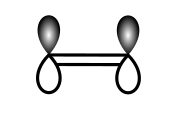
\includegraphics[scale=1]{./structures/exercise_1/ethylene/1.png}
			\captionof*{figure}{$\varepsilon = \alpha + \beta$}
			\end{minipage} & 
			\begin{minipage}[t]{0.11\linewidth}
			\setlength{\abovecaptionskip}{0.5em}
			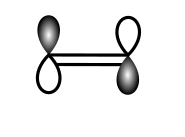
\includegraphics[scale=1]{./structures/exercise_1/ethylene/2.png}
			\captionof*{figure}{$\varepsilon = \alpha - \beta$}
			\end{minipage}
		\end{tabular}				
		\captionof{figure}{Phase diagrams of these H{\"u}ckel MOs. Black bubbles mean plus phase while white ones mean minus phase. The color is used just for determining relative phase.}\label{fig:phase_diagram_2}
		\end{center}